\section{Experimental methodology}\label{sec:experiments}
The experiment measures the cost of checking a declared operational
explanation alongside the cost of direct final-word verification.
It evaluates a Python reference implementation, not code extracted
from Lean. All data discussed here were generated by a new,
prespecified campaign on 23 September 2026. The earlier manuscript's
outputs remain in a separate, unchanged directory and are not used in
these figures or tables. The configuration, individual matrix adjacency
lists and hashes, random seeds, per-trial outcomes, repeated timings,
source snapshots and environment metadata accompany the artifact.

\paragraph{Graphs and observations.}
Both constructions have variable degree three and check degree six,
so $m=n/2$. The regular construction samples uniform socket
permutations and rejects nonsimple graphs. The PEG variant chooses
maximum graph distance and then minimum check degree, subject to a
check-capacity constraint, and restarts if a construction gets stuck.
It is an explicitly specified variant of the progressive edge-growth
method \cite{HuEleftheriouArnold2005PEG}; we do not assume it samples a
uniform ensemble or reproduces another implementation's finite-length
performance. Each family uses $n\in\{128,256,512,1024\}$ and three
independently seeded matrices per size, giving 24 matrices. Each matrix
is reused across the channel conditions. Matrix generation, validation,
dense conversion and kernel-basis construction are measured once per
matrix and excluded from per-observation decoding times.

The clean campaign uses $\varepsilon\in\{0.30,0.40,0.50\}$ and ten
observations per matrix and erasure probability, giving 720 trials.
For each trial, a uniformly sampled coefficient vector in a computed
kernel basis generates a uniformly sampled codeword. Erasures are
independent Bernoulli variables. Distinct random streams generate the
codeword, erasures, visible flips and measurement order. Their seeds
are 64-bit prefixes of SHA-256 hashes of a fixed base seed and the
complete trial/stream labels; the artifact records the exact encoding
and checks for collisions in the executed grid.

Corruption trials use both families, $n\in\{256,512\}$,
$\varepsilon\in\{0.40,0.55\}$ and flip probabilities
$\delta\in\{0.001,0.01\}$, with three matrices and ten observations
per condition, giving 480 trials. A flip applies only at a nonerased
coordinate. We record the realized number of flips, since a positive
$\delta$ does not imply any bit changed. Compatibility means existence
of a codeword consistent with the supplied, possibly corrupted,
observation. Incompatibility is accompanied by a checked separator.

\paragraph{Compared operations and timing.}
We measure peeling only, Gaussian elimination only, hybrid decoding,
hybrid decoding with certificate checking, and independent direct
word verification. All algebraic pipelines use the same integer-bitset,
first-available-pivot elimination engine and row-transformation tracking.
The hybrid without checking still constructs its certificate; the
comparison isolates execution of the checker and does not measure a
producer optimized to avoid witness construction. Peeling alone is
incomplete on stopping sets. Direct verification receives an already
produced word and is a verification operation, not a decoder or an
infeasibility test.

Each per-observation operation includes its own required initialization
on a prevalidated adjacency structure. There is one warmup per operation
and three timed repetitions in deterministically randomized order.
Comparator times are within-trial medians. The certified pipeline also
records initialization, peeling, residual construction, elimination,
witness extraction, back substitution, other producer work and checking.
For its stage decomposition we select the actual repetition with median
internal total time; this preserves the identity
\[
 T_{\mathrm{total}}=T_{\mathrm{decode}}+T_{\mathrm{check}}.
\]
Here $T_{\mathrm{decode}}$ includes construction of the certificate.
The internal $T_{\mathrm{check}}$ also includes the producer wrapper's
assertion that the checker returns its proposed word; standalone replay
timings exclude that wrapper comparison.
We report both $R_{\mathrm{relative}}=T_{\mathrm{check}}/
T_{\mathrm{decode}}$ and $R_{\mathrm{fraction}}=
T_{\mathrm{check}}/T_{\mathrm{total}}$. A mean of per-trial ratios is
not a ratio of mean times; the condition-summary CSV provides both.
The outer comparator timer also measures call overhead, so it is not
silently identified with an internal stage timer.

A separate checker experiment uses 15 additional regular matrices:
three each at $n\in\{256,512,1024,2048,4096\}$, six observations per
matrix, $\varepsilon=0.40$, and five randomized timing repetitions.
These 90 trials use the all-zero transmitted word to isolate checking;
no recovery inference is drawn from them. Each checker is called once
for validation before timing. Sparse replay, dense replay and direct
checking receive the same instance and resulting completion; the two
replay checkers receive the same certificate. Dense input conversion
is excluded, but the dense checker scans its matrix during checking.

Memory is measured separately using \texttt{tracemalloc}: peak
incremental Python-tracked allocation during a call, not resident set
size or total artifact storage. One observation per matrix and clean
channel condition, and one per scaling matrix, is profiled. The
preexisting graph, dense matrix and certificate are outside that
incremental measurement. The run used an Apple M3 Pro (11 reported
logical CPUs, approximately 18\,GiB RAM), macOS 27.0 arm64, Python
3.12.14, NumPy 2.3.5, pandas 2.2.3 and Matplotlib 3.10.7, with
\texttt{perf\_counter} as the clock. Exact package versions are pinned.

\paragraph{Outcomes and uncertainty.}
Completion means acceptance of a success certificate. Exact recovery
compares its word with the sampled transmitted word. Uniqueness is
$|U|-\operatorname{rank}(H_U)=0$, conditional on compatibility.
These meanings are those of Section~\ref{sec:certificates}.
Failure-certificate acceptance is recorded separately from completion.
Each displayed condition at a fixed family, size and channel parameter
has three matrix realizations and ten observations per matrix.
Intervals in the supplementary data use 2,000 bootstrap resamples of
matrix means, retaining within-matrix dependence. The scaling fit is
ordinary least squares of log mean time against log blocklength;
its interval resamples the three matrix means independently within each
size. These descriptive intervals have limited ensemble resolution:
three matrices do not support strong distributional claims, even when
many channel observations or timing repetitions are available.

\section{Experimental results and interpretation}\label{sec:results}
% Generated only from raw campaign CSVs. See results.json and condition_summary.csv.
The new campaign contains 720 clean-channel trials on 24 matrices, 480 corruption trials, and 90 separate checker-scaling trials. Valid completion was obtained in 1.000 of clean trials, whereas exact recovery occurred in 0.781; 174 clean residual systems were nonunique. Among 251 inputs with at least one visible flip, 100 remained compatible.

A clean observation always has the transmitted codeword as a compatible
completion. The 100\% observed completion rate is therefore implementation
evidence, not an additional recovery theorem.
The exact counts are 562 exact recoveries and 546 unique completions
among the 720 clean trials. All uniquely completable clean observations
were recovered exactly. The remaining exact recoveries occurred when
the chosen completion happened to equal the transmitted word in a
nonunique system. Figure~\ref{fig:completion} separates these events.
Its fixed mixture pools the four declared sizes with equal trial
counts; it is not a threshold estimate for either ensemble.

\begin{figure}[t]
\centering
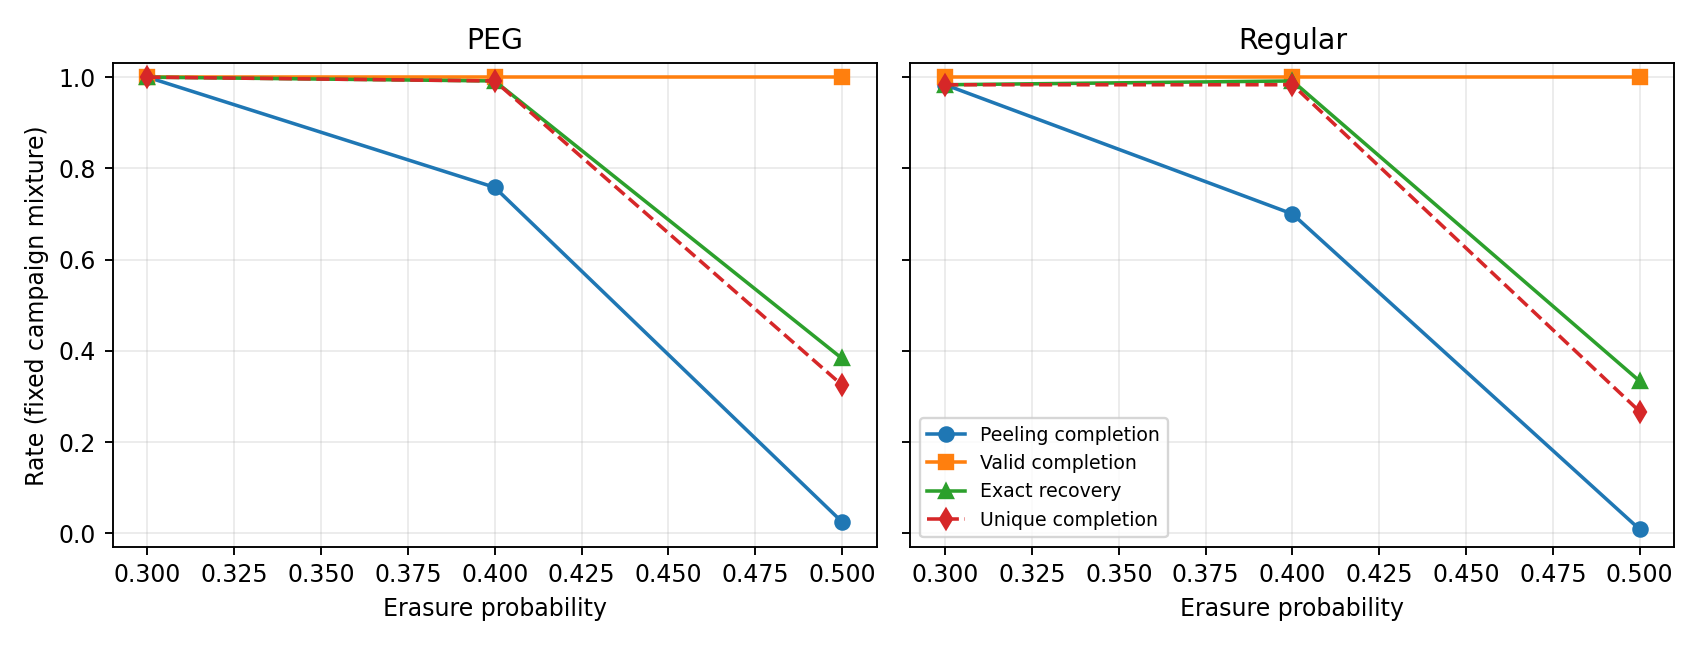
\includegraphics[width=\textwidth]{publication_outputs/fig_completion.png}
\caption{Clean-channel outcomes, displayed separately for each graph
construction. Each point pools 120 trials: four sizes, three matrices
per size and ten observations per matrix at the stated erasure
probability. Valid completion, exact recovery, uniqueness and peeling
completion answer different questions.}
\label{fig:completion}
\end{figure}

\begin{table}
\centering
\small
\setlength{\tabcolsep}{3pt}
\caption{New campaign at erasure probability 0.40: three matrices and ten trials per matrix. C/D is the internal check stage divided by decode time, averaged per trial. The check stage includes comparing checker and producer words.}
\label{tab:new-experiments}
\begin{tabular}{lrrrrrrr}
\toprule
Family & n & Trials & Trace & Residual & Check ms & Direct ms & Mean C/D \\
\midrule
PEG & 128 & 30 & 35.767 & 16.400 & 0.119 & 0.092 & 1.107 \\
PEG & 256 & 30 & 77.367 & 22.233 & 0.241 & 0.186 & 1.147 \\
PEG & 512 & 30 & 190.033 & 11.933 & 0.527 & 0.366 & 1.415 \\
PEG & 1024 & 30 & 389.100 & 22.900 & 1.109 & 0.741 & 1.376 \\
Regular & 128 & 30 & 33.000 & 18.833 & 0.119 & 0.094 & 0.990 \\
Regular & 256 & 30 & 84.500 & 15.900 & 0.247 & 0.184 & 1.243 \\
Regular & 512 & 30 & 174.133 & 32.467 & 0.530 & 0.375 & 1.229 \\
Regular & 1024 & 30 & 377.933 & 33.567 & 1.102 & 0.739 & 1.346 \\
\bottomrule
\end{tabular}
\end{table}

Table~\ref{tab:new-experiments} filters exactly $\varepsilon=0.40$ and
$\delta=0$; no other erasure probabilities enter its averages.
Trace and residual columns are mean numbers of variables. The check-stage column
reports the internal checker stage of the selected certified repetition;
direct checking reports its separately timed median. For these 240
trials, the mean per-trial relative overhead was 1.232, whereas the mean
checker fraction of total time was 0.522. The checker is therefore a
substantial fraction of the measured pipeline, not negligible overhead.
The corresponding ratios of mean times are 0.859 and 0.462; their
difference from the mean ratios reflects variation across trials. The
complete condition CSV also reports the other channel conditions.

\begin{figure}[t]
\centering
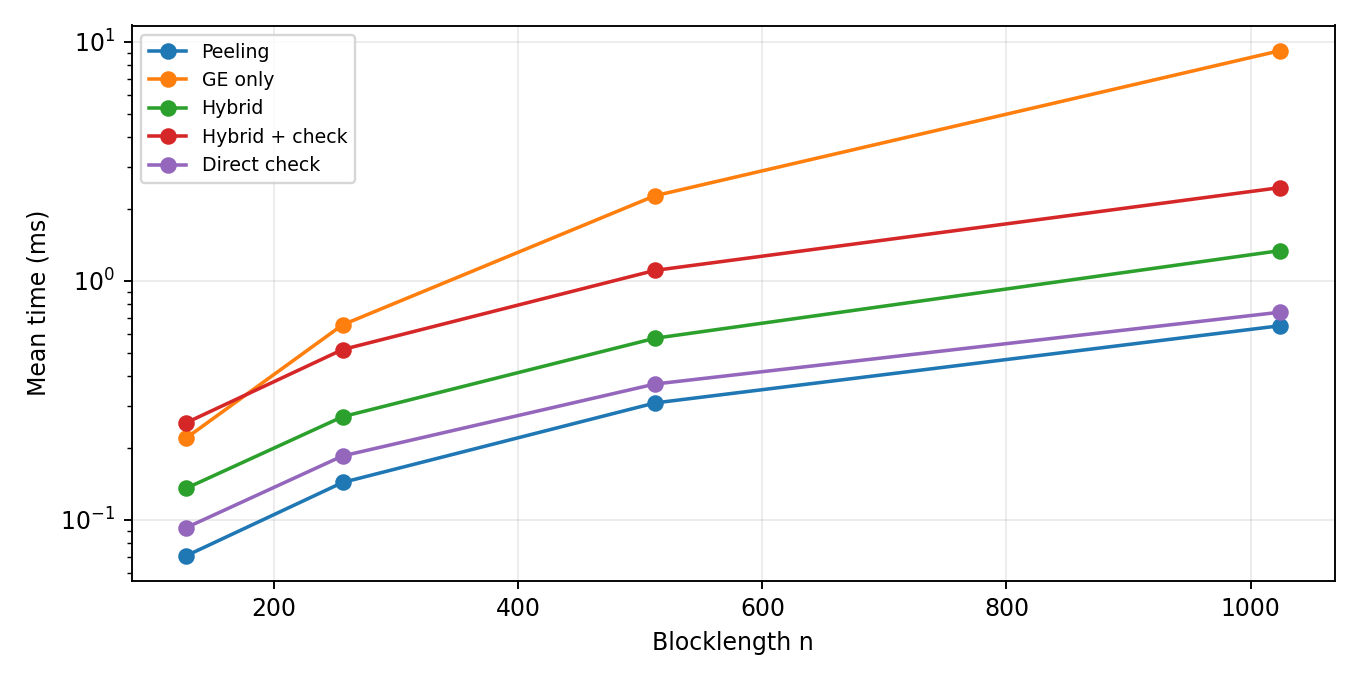
\includegraphics[width=.85\textwidth]{publication_outputs/fig_comparators.png}
\caption{Mean within-trial median times at $\varepsilon=0.40$.
Each size pools 60 observations across both families, with three
matrices per family and ten observations per matrix. Peeling alone may leave
unknowns. Direct checking assumes an already supplied word. Its time
must not be interpreted as a competing decoding latency.}
\label{fig:comparators}
\end{figure}
Figure~\ref{fig:comparators} uses the same algebraic engine across
GE-only and hybrid pipelines. It describes this engine and finite set
of graphs, without attributing a universal speed advantage to the
hybrid strategy or to SELL. Table~\ref{tab:runtime-stages} separates stage means in the same fixed
mixture. Detailed measurements are retained for every observation, so
witness construction and checker cost remain separable from residual
elimination.
\begin{table}
\centering
\small
\setlength{\tabcolsep}{3pt}
\caption{Mean certified runtime stages in milliseconds at erasure probability 0.40, pooled equally over the two named families: six matrices and 60 trials per size. Witness is final vector extraction; row-transform tracking is included in GE. Other includes parsing, output reconstruction and timing overhead; Check includes comparing checker and producer words.}
\label{tab:runtime-stages}
\begin{tabular}{lrrrrrrrr}
\toprule
n & Init & Peel & Residual & GE & Witness & Backsub & Other & Check \\
\midrule
128 & 0.0134 & 0.0137 & 0.0113 & 0.0494 & 0.0001 & 0.0026 & 0.0440 & 0.1187 \\
256 & 0.0266 & 0.0310 & 0.0200 & 0.1019 & 0.0001 & 0.0029 & 0.0872 & 0.2441 \\
512 & 0.0576 & 0.0774 & 0.0380 & 0.2269 & 0.0001 & 0.0035 & 0.1714 & 0.5285 \\
1024 & 0.1229 & 0.1867 & 0.0726 & 0.6213 & 0.0001 & 0.0047 & 0.3375 & 1.1054 \\
\bottomrule
\end{tabular}
\end{table}


\begin{figure}[t]
\centering
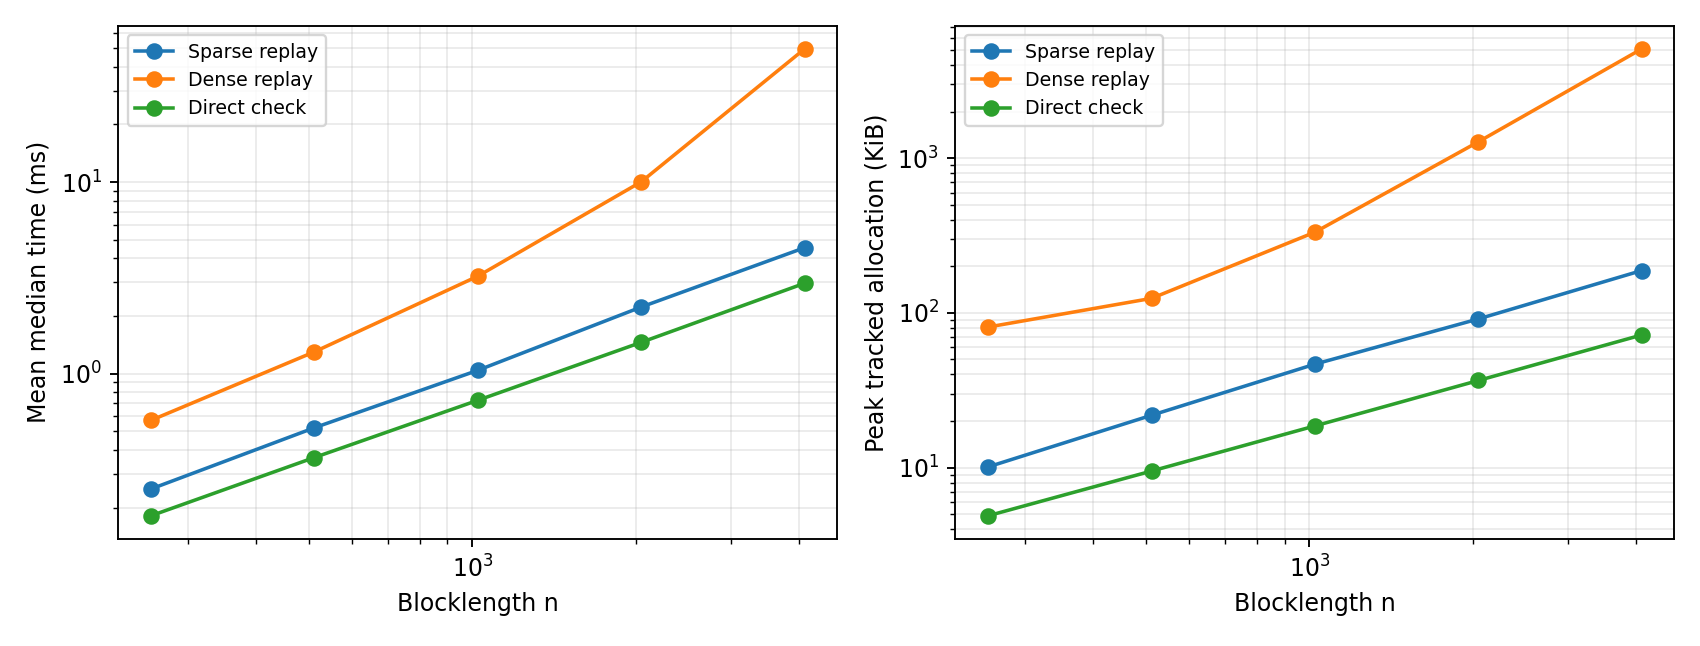
\includegraphics[width=\textwidth]{publication_outputs/fig_checker_scaling.png}
\caption{Independent checker scaling experiment. Time points average
18 within-trial medians (three matrices and six observations); allocation
points average three separately profiled calls, one per matrix. Both
axes of each panel are logarithmic. Allocations exclude preexisting
inputs. The dense and sparse replay implementations check the same
certificates.}
\label{fig:scaling}
\end{figure}
At $n=4096$, mean sparse replay took 4.546\,ms, direct checking
2.966\,ms, and dense replay 49.574\,ms. Corresponding incremental
tracked peaks were approximately 188, 72 and 5094\,KiB.
Thus direct checking was faster and used less additional memory than
trace replay. Both establish the same final parity and visible-coordinate
agreement. Replay additionally checks that each declared assignment is
justified by a degree-one constraint in the preceding operational state.
The measured costs compare complete checker implementations; they do not
isolate the cost of an individual replay step. The fitted time exponents were
1.046 (95\% matrix-bootstrap interval $[1.033,1.062]$) for sparse replay,
1.006 ($[1.003,1.008]$) for direct checking, and
1.583 ($[1.555,1.617]$) for dense replay. The observed sparse exponent
is slightly above one; we do not force a linear fit or treat its
interval as a proof of asymptotic complexity. The abstract sparse bound
in Section~\ref{sec:cost} instead follows from counting incidence
visits in the stated model. Dense scans and Python/runtime effects
prevent identifying every measured implementation with that model.

\begin{figure}[t]
\centering
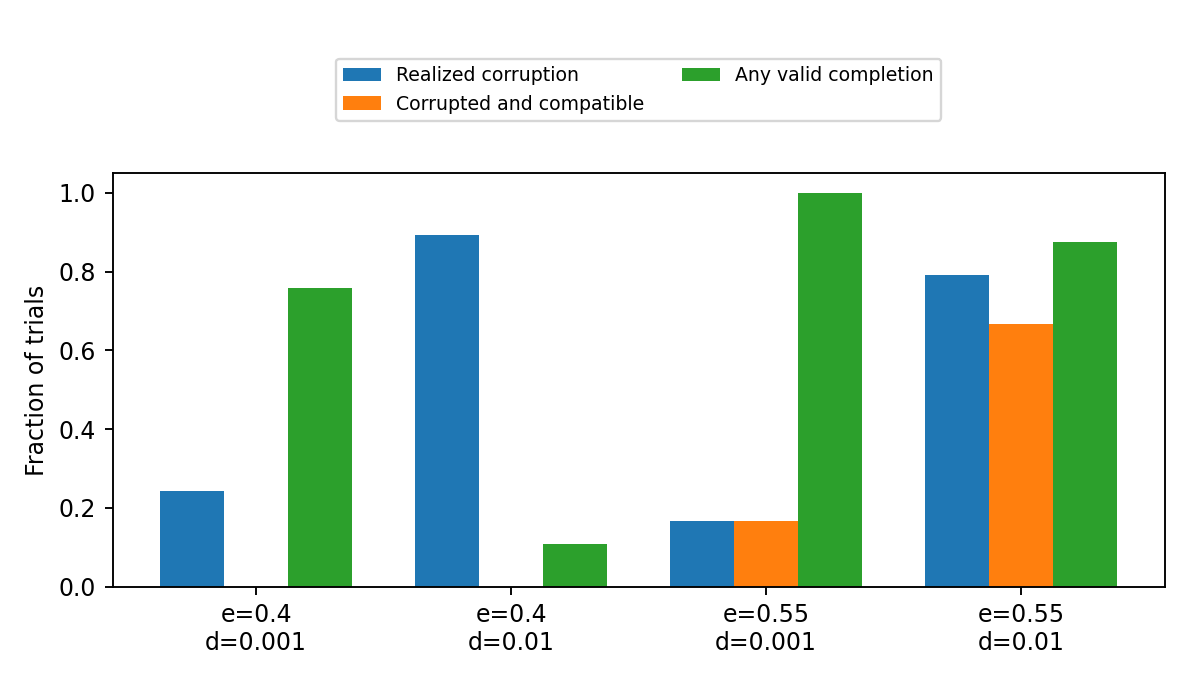
\includegraphics[width=.82\textwidth]{publication_outputs/fig_corruption.png}
\caption{Visible-bit corruption: each group has 120 trials, pooling
two families, two sizes, three matrices and ten observations per
matrix. All bars use that same denominator. ``Corrupted and compatible''
is not conditional on realized corruption; it is a subset of the
``Realized corruption'' bar.}
\label{fig:corruption}
\end{figure}
Of 480 corruption trials, 229 realized no flip. Of the 251 with at
least one flip, 151 were incompatible and yielded accepted failure
certificates; 100 remained compatible and yielded accepted success
certificates. In this fixed campaign, incompatibility exposed
$151/251\approx60.2\%$ of actually corrupted inputs. The remaining
$100/251\approx39.8\%$ cannot be rejected merely for lacking a
completion. Figure~\ref{fig:corruption} uses unconditional trial
fractions, so its bars must not be confused with these conditional
rates. This is algebraic compatibility detection, not a guarantee
against every BEC violation.

\paragraph{Reproducibility and negative evidence.}
The runner checks the complete declared trial grid, preserves all
outcomes, checks matrix fingerprints and records raw-data hashes.
An analysis-stage serialization error and a missing table-rendering
dependency were repaired after all measurements had finished; the
complete original measurements were retained and only analysis was
rerun. Both the executed measurement source and corrected analysis
source are identifiable in the artifact. Tables and figures are
generated from the CSVs by the script and reproducibility notebook.
Finite adversarial tests include malformed domains and certificate
lengths, altered values and indices, invalid orderings, and valid
partial or independently commuting traces. Their observed acceptance
or rejection is test evidence, not a theorem about the Python runtime.
The direct-check advantage, nonunique completions, compatible corruption
and finite-size superlinear fits are retained rather than filtered
from the scientific conclusions.
